\PassOptionsToPackage{unicode=true}{hyperref} % options for packages loaded elsewhere
\PassOptionsToPackage{hyphens}{url}
%
\documentclass[10pt,]{article}
\usepackage{lmodern}
\usepackage{amssymb,amsmath}
\usepackage{ifxetex,ifluatex}
\usepackage{fixltx2e} % provides \textsubscript
\ifnum 0\ifxetex 1\fi\ifluatex 1\fi=0 % if pdftex
  \usepackage[T1]{fontenc}
  \usepackage[utf8]{inputenc}
  \usepackage{textcomp} % provides euro and other symbols
\else % if luatex or xelatex
  \usepackage{unicode-math}
  \defaultfontfeatures{Ligatures=TeX,Scale=MatchLowercase}
    \setmainfont[]{Arial}
\fi
% use upquote if available, for straight quotes in verbatim environments
\IfFileExists{upquote.sty}{\usepackage{upquote}}{}
% use microtype if available
\IfFileExists{microtype.sty}{%
\usepackage[]{microtype}
\UseMicrotypeSet[protrusion]{basicmath} % disable protrusion for tt fonts
}{}
\IfFileExists{parskip.sty}{%
\usepackage{parskip}
}{% else
\setlength{\parindent}{0pt}
\setlength{\parskip}{6pt plus 2pt minus 1pt}
}
\usepackage{hyperref}
\hypersetup{
            pdftitle={Risk of incident prostate cancer risk, weighted by survival to 1985},
            pdfborder={0 0 0},
            breaklinks=true}
\urlstyle{same}  % don't use monospace font for urls
\usepackage[margin=3cm]{geometry}
\usepackage{graphicx,grffile}
\makeatletter
\def\maxwidth{\ifdim\Gin@nat@width>\linewidth\linewidth\else\Gin@nat@width\fi}
\def\maxheight{\ifdim\Gin@nat@height>\textheight\textheight\else\Gin@nat@height\fi}
\makeatother
% Scale images if necessary, so that they will not overflow the page
% margins by default, and it is still possible to overwrite the defaults
% using explicit options in \includegraphics[width, height, ...]{}
\setkeys{Gin}{width=\maxwidth,height=\maxheight,keepaspectratio}
\setlength{\emergencystretch}{3em}  % prevent overfull lines
\providecommand{\tightlist}{%
  \setlength{\itemsep}{0pt}\setlength{\parskip}{0pt}}
\setcounter{secnumdepth}{0}
% Redefines (sub)paragraphs to behave more like sections
\ifx\paragraph\undefined\else
\let\oldparagraph\paragraph
\renewcommand{\paragraph}[1]{\oldparagraph{#1}\mbox{}}
\fi
\ifx\subparagraph\undefined\else
\let\oldsubparagraph\subparagraph
\renewcommand{\subparagraph}[1]{\oldsubparagraph{#1}\mbox{}}
\fi

% set default figure placement to htbp
\makeatletter
\def\fps@figure{htbp}
\makeatother

\PassOptionsToPackage{no-math}{fontspec}

%---------------------------------------------------------------------------
% Kevin's style file
%---------------------------------------------------------------------------
\usepackage{ifxetex,ifluatex}

%---------------------------------------------------------------------------
% General
%---------------------------------------------------------------------------

% When testing
% \usepackage{lipsum}

% Line numbering
\usepackage{lineno}

% Usage
	% \linenumbers
	% \modulolinenumbers[2]
	% \renewcommand\thelinenumber{\color{red}\Roman{linenumber}}
	% \begin{linenumbers}  \end{linenumbers}


\usepackage{setspace}
%\doublespacing

\usepackage{outlines}
\usepackage{enumitem}
\setenumerate[4]{label=\alph*).}

\setlength\parindent{0pt} % Removes all indentation from paragraphs

% \renewcommand{\thesection}{\Alph{section}} % Lettered, not numbered sections
%\usepackage{sectsty} % Allows customizing section commands
%\allsectionsfont{\centering \normalfont\scshape} % Make all sections centered, the default font and small caps
%\numberwithin{equation}{section} % Number equations within sections
%\numberwithin{figure}{section} % Number figures within sections
%\numberwithin{table}{section} % Number tables within sections


\usepackage{multicol}
\setlength{\columnsep}{15pt}
\newlength\Colsep

\usepackage{wrapfig}

%---------------------------------------------------------------------------
% Header/footer
%---------------------------------------------------------------------------
\usepackage{fancyhdr}
\pagestyle{fancyplain}
\fancyhead[L]{}
\fancyhead[C]{}
\fancyhead[R]{}
% \fancyfoot[L]{}
% \fancyfoot[C]{}
% \fancyfoot[R]{\thepage}
\renewcommand{\headrulewidth}{0pt}
% \renewcommand{\footrulewidth}{0pt}
% \setlength{\headheight}{15pt}

%---------------------------------------------------------------------------
% Tables, figures, images
%---------------------------------------------------------------------------
\usepackage{color}
% \usepackage[usenames,dvipsnames]{xcolor}
\usepackage{xparse}
\usepackage{xhfill}
\ifnum 0\ifxetex 1\fi\ifluatex 1\fi=0
% Requires pdfTeX
\usepackage{linegoal}
\fi

\usepackage{longtable}
\setlength{\LTcapwidth}{\textwidth}
\usepackage{xtab, booktabs}
\usepackage{multirow}
\usepackage[flushleft]{threeparttable} % Suzanne's

\usepackage{float} % Check code chunks section for floatrow

\ifluatex
% requires lualatex
\usepackage{pgf}
\fi
\usepackage{tikz}% Probability trees and flow charts and the like
\usetikzlibrary{
graphs,
arrows,
automata
%trees,
%shapes,
%decoration,
%backgrounds,
%petri
}
\ifluatex
% requires lualatex
\usetikzlibrary{graphdrawing}
\fi

\usepackage{graphicx}
% \usepackage{grffile}
% \usepackage{subcaption}
% For tables and figures in parts %%%%
\usepackage{caption}
% \DeclareCaptionLabelFormat{cont}{#1~#2\alph{ContinuedFloat}}
% \captionsetup[ContinuedFloat]{labelformat=cont}
%\graphicspath{ {file.path.here} }

% Set column widths in tabular environment!
\usepackage{array}
\newcommand{\PreserveBackslash}[1]{\let\temp=\\#1\let\\=\temp}
\newcolumntype{C}[1]{>{\PreserveBackslash\centering}p{#1}}
\newcolumntype{R}[1]{>{\PreserveBackslash\raggedleft}p{#1}}
\newcolumntype{L}[1]{>{\PreserveBackslash\raggedright}p{#1}}

% STATA output for `estout` package
\def\sym#1{\ifmmode^{#1}\else\(^{#1}\)\fi}


%---------------------------------------------------------------------------
% Code chunks and color
%---------------------------------------------------------------------------
% \usepackage{cprotect}
\usepackage{listings} % for code
\usepackage{tcolorbox}
\NewDocumentCommand{\framecolorbox}{oommm}
 {% #1 = width (optional)
  % #2 = inner alignment (optional)
  % #3 = frame color
  % #4 = background color
  % #5 = text
  \IfValueTF{#1}
   {\IfValueTF{#2}
    {\fcolorbox{#3}{#4}{\makebox[#1][#2]{#5}}}
    {\fcolorbox{#3}{#4}{\makebox[#1]{#5}}}%
   }
   {\fcolorbox{#3}{#4}{#5}}%
 }


%\definecolor{codegreen}{rgb}{0,0.6,0}
%\definecolor{codegray}{rgb}{0.5,0.5,0.5}
%\definecolor{codepurple}{rgb}{0.58,0,0.82}
%\definecolor{backcolour}{rgb}{0.95,0.95,0.92}
%
%\lstdefinestyle{mystyle}{
%backgroundcolor=\color{backcolour},
%commentstyle=\color{codegreen},
%keywordstyle=\color{magenta},
%numberstyle=\tiny\color{codegray},
%stringstyle=\color{codepurple},
%basicstyle=\footnotesize,
%breakatwhitespace=false,
%breaklines=true,
%captionpos=b, keepspaces=true, numbers=left, numbersep=5pt, showspaces=false,
%showstringspaces=false, showtabs=false, tabsize=2 }
%
%\lstset{style=mystyle}


\usepackage{hyperref}
\hypersetup{unicode=true,
            pdfauthor={Kevin Chen},
            pdfborder={0 0 0},
            breaklinks=true}

% Code chunk captions and references
% \usepackage{floatrow} %interferes with float package
% \floatsetup[figure]{capposition=top}
% \floatsetup[table]{capposition=top}
% \DeclareNewFloatType{chunk}{placement=H, fileext=chk, name=}
% \captionsetup{options=chunk}
% \renewcommand{\thechunk}{Chunk~\arabic{chunk}}
% \makeatletter
% \@addtoreset{chunk}{section}
% \makeatother

% Usage in R
% library(knitr)
% oldSource <- knit_hooks$get("source")
% knit_hooks$set(source = function(x, options) {
%   x <- oldSource(x, options)
%   x <- ifelse(!is.null(options$ref), paste0("\\label{", options$ref,"}", x), x)
%   ifelse(!is.null(options$codecap), paste0("\\captionof{chunk}{", options$codecap,"}", x), x)
% })

%---------------------------------------------------------------------------
% Including R chunks (LaTex)
%---------------------------------------------------------------------------

\lstloadlanguages{R} % Load R syntax for listings, for a list of other languages supported see: ftp://ftp.tex.ac.uk/tex-archive/macros/latex/contrib/listings/listings.pdf
\definecolor{gray}{rgb}{0.5,0.5,0.5}
\definecolor{green}{rgb}{0,0.6,0}
\definecolor{mauve}{rgb}{0.58,0,0.82}
\definecolor{maroon}{rgb}{0.3,0.1,0.9}
\lstset{
language=R,
basicstyle=\scriptsize\ttfamily,
commentstyle=\ttfamily\color{gray},
numbers=left,
numberstyle=\ttfamily\color{gray}\footnotesize,
stepnumber=1,
numbersep=5pt,
backgroundcolor=\color{white},
showspaces=false,
showstringspaces=false,
showtabs=false,
frame=single,
tabsize=2,
captionpos=b,
breaklines=true,
breakatwhitespace=false,
% title=\lstname,
escapeinside={},
keywordstyle=\ttfamily\color{green},
stringstyle=\ttfamily\color{mauve},
identifierstyle=\color{blue},
morekeywords={}
}

% Usage
	% For use in LaTex or Sweave:
	% \lstinputlisting[language=R]{Script.R}

%---------------------------------------------------------------------------
% Typographical addendum
%---------------------------------------------------------------------------
% \usepackage{hologo}
\ifnum 0\ifxetex 1\fi\ifluatex 1\fi=0 % if pdftex
% TIPA (not compatible with fontspec)
\usepackage{tipx}
\fi
\usepackage{marvosym,epsdice}
\usepackage{physics}
\usepackage{amsmath,amsfonts,amsthm,amssymb}
\usepackage{mathtools} \mathtoolsset{showonlyrefs}
\usepackage{bm} % greek no good in lualatex
\usepackage{MnSymbol} % good-looking extended math symbols
% \usepackage{lilyglyphs} % Extended music symbols (needs XeLaTex of LuaTex)
\usepackage{dsfont} % for cool indicator
\usepackage{textcomp} % because unicode and hyperref may have issues

\makeatletter
\newcommand*{\indep}{%
  \mathbin{%
    \mathpalette{\@indep}{}%
  }%
}
\newcommand*{\nindep}{%
  \mathbin{%                   % The final symbol is a binary math operator
    \mathpalette{\@indep}{\not}% \mathpalette helps for the adaptation
                               % of the symbol to the different math styles.
  }%
}
\newcommand*{\@indep}[2]{%
  % #1: math style
  % #2: empty or \not
  \sbox0{$#1\perp\m@th$}%        box 0 contains \perp symbol
  \sbox2{$#1=$}%                 box 2 for the height of =
  \sbox4{$#1\vcenter{}$}%        box 4 for the height of the math axis
  \rlap{\copy0}%                 first \perp
  \dimen@=\dimexpr\ht2-\ht4-.2pt\relax
      % The equals symbol is centered around the math axis.
      % The following equations are used to calculate the
      % right shift of the second \perp:
      % [1] ht(equals) - ht(math_axis) = line_width + 0.5 gap
      % [2] right_shift(second_perp) = line_width + gap
      % The line width is approximated by the default line width of 0.4pt
  \kern\dimen@
  {#2}%
      % {\not} in case of \nindep;
      % the braces convert the relational symbol \not to an ordinary
      % math object without additional horizontal spacing.
  \kern\dimen@
  \copy0 %                       second \perp
}
\makeatother

% limits underneath
\DeclareMathOperator*{\argminA}{arg\,min} % Jan Hlavacek
\DeclareMathOperator*{\argminB}{argmin}   % Jan Hlavacek
\DeclareMathOperator*{\argminC}{\arg\min}   % rbp
\newcommand{\argminD}{\arg\!\min} % AlfC
\newcommand{\argminE}{\mathop{\mathrm{argmin}}}          % ASdeL
\newcommand{\argminF}{\mathop{\mathrm{argmin}}\limits}   % ASdeL

\newcommand{\horrule}[1]{\rule{\linewidth}{#1}} % Create horizontal rule command with 1 argument of height

\newcommand{\Prob}[2][]{ \mathbb{P}_{#1} \left\{ {#2} \right\}} % make a function for bb bold P with curly braces

\newcommand{\E}[2][]{ \mathbb{E}_{#1}\left[ {#2} \right]} % make a function for expectation

\newcommand{\Var}[2][]{ \mathrm{Var}_{#1}\left( {#2} \right)} % function for Var

\newcommand{\Cov}[2][]{ \mathrm{Cov}_{#1}\left( {#2} \right)} % function for Covar

\newcommand{\lik}[2][]{ \mathrm{lik}_{#1}\left( {#2} \right)} % function for lik

\newcommand{\Ind}[2][]{\mathds{1}_{#1}\left[ {#2} \right]} % function for Indicator

\DeclarePairedDelimiter\Abs{\lvert}{\rvert}

\DeclarePairedDelimiter\dis{\lVert}{\rVert}

% Swap the definition of \abs* and \norm*, so that \abs
% and \norm resizes the size of the brackets, and the
% starred version does not.
\makeatletter
\let\oldabs\abs
\def\abs{\@ifstar{\oldabs}{\oldabs*}}

\let\olddis\dis
\def\dis{\@ifstar{\olddis}{\olddis*}}
\makeatother

% For typesetting the "distributed as" symbol
% example of use:
% X \distras{H_0} Y
\makeatletter
\newcommand{\distas}[1]{\mathbin{\overset{#1}{\kern\z@\sim}}}%
\newsavebox{\mybox}\newsavebox{\mysim}
\newcommand{\distras}[1]{%
  \savebox{\mybox}{\hbox{\kern3pt$\scriptstyle#1$\kern3pt}}%
  \savebox{\mysim}{\hbox{$\sim$}}%
  \mathbin{\overset{#1}{\kern\z@\resizebox{\wd\mybox}{\ht\mysim}{$\sim$}}}%
}
\makeatother

%---------------------------------------------------------------------------
% Environment commands for Markdown
%---------------------------------------------------------------------------
\usepackage{pdflscape}
\newcommand{\blandscape}{\begin{landscape}}
\newcommand{\elandscape}{\end{landscape}}

\newcommand{\bcenter}{\begin{center}}
\newcommand{\ecenter}{\end{center}}

\newcommand{\bsinglespace}{\begin{singlespace}}
\newcommand{\esinglespace}{\end{singlespace}}

\newcommand\startsupplement{%
    \makeatletter
       \setcounter{table}{0}
       \renewcommand{\thetable}{S\arabic{table}}
       \setcounter{figure}{0}
       \renewcommand{\thefigure}{S\arabic{figure}}
    \makeatother}

%---------------------------------------------------------------------------
% Bibliography
%---------------------------------------------------------------------------
% \usepackage[backend=bibtex]{biblatex}

%---------------------------------------------------------------------------
% Usage
%---------------------------------------------------------------------------

% For use in LaTex or Sweave:
% \input{/Users/kevinchen/Documents/computing/HeadRs/StatHead.tex}

% An example YAML header for Rmd
% ---
% title: "Stat 2"
% author: "Kevin Chen"
% date: \today
% output:
%   pdf_document:
%      # keep_tex: true
%     #  pandoc_args: [
%     #   "-V", "classoption=twocolumn"
%     # ]
%      includes:
%         in_header: /Users/kevinchen/Documents/computing/HeadRs/StatHead.tex
% bibliography: /Users/kevinchen/Documents/2017 Fa/245/MV_FinalProj/mv_final.bib
% csl: /Users/kevinchen/Documents/computing/HeadRs/AMA.csl
% geometry: margin=2cm, bottom=2.5cm
% ---


%---------------------------------------------------------------------------
% Fonts
%---------------------------------------------------------------------------

%\usepackage[T1]{fontenc} % Use 8-bit encoding that has 256 glyphs
%\usepackage[utf8]{inputenc}
% Latin Modern Roman
% \usepackage{lmodern}
%\usepackage{fourier} % Use the Adobe Utopia font for the document - comment this line to return to the LaTeX default

\ifluatex
%%%%%%%%%%%%%%%%%%%%%%%%%%%
% For Arial (with lualatex)
%%%%%%%%%%%%%%%%%%%%%%%%%%%
\usepackage[no-math]{fontspec}
% \setmainfont{Arial}[
% % Options below necessary for Windows
% 	% Extension = .ttf,
% 	% UprightFont = *,
% 	% BoldFont = *bd,
% 	% ItalicFont = *i,
% 	% BoldItalicFont = *bi
% 	]
% In YAML
% ---
% mainfont: Arial
% ---
% \usepackage{lualatex-math}

% Math as text, but numerals do not mpa well becuase
% mathastext clahes with unicode-math
% \usepackage[italic]{mathastext}
%%%%%%%%%%%%%%%%%%%%%%%%%%%
\fi
\usepackage{etoolbox}
\makeatletter
\providecommand{\subtitle}[1]{% add subtitle to \maketitle
  \apptocmd{\@title}{\par {\large #1 \par}}{}{}
}
\makeatother

\title{Risk of incident prostate cancer risk, weighted by survival to 1985}
\providecommand{\subtitle}[1]{}
\subtitle{GM-UAW Cohort Study}
\author{}
\date{\vspace{-2.5em}\today}

\begin{document}
\maketitle

\renewcommand\arraystretch{1.1}
\onehalfspacing

\hypertarget{the-problem}{%
\section{The problem}\label{the-problem}}

The Cohort includes all persons who have worked at least 3 years and
were hired in the years 1938 through 1981. However, follow-up for cancer
incidence (Michigan Cancer Registry) does not begin until 1985. Not all
who entered the cohort prior to 1985 were still at-risk of the outcome
in 1985. Loss to follow-up may have been differential by underlying
health. In particular, healthier individuals may have had lower exposure
and a greater probability of surviving to 1985 outcome-free. In this
case, the resulting population at-risk in 1985 would be the result of
the so-called healthy worker survivor bias.\textsuperscript{1} (There
may also be those who have already experienced incident cancer prior to
1985, but were not recorded as such, but this outcome misclassification
problem is not the focus of this analysis.)

\begin{figure}
\caption{Adapted from Figure 6c in Hernán et al. (2004). Take $L$, $E$, $C$, and $Y$ to represent underlying health, occupational exposure, censoring, and cancer incidence, respectively.}
\centering
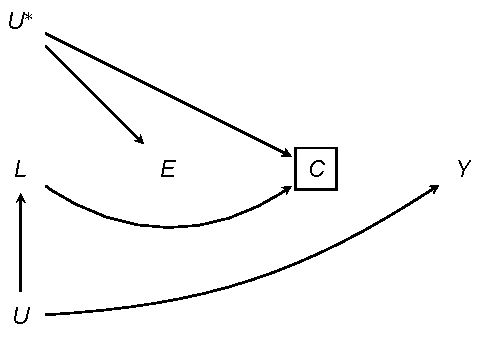
\includegraphics{"/Users/kevinchen/eisen/GM/reports/left truncation/prostate cancer/resources/dag.pdf"}
\end{figure}

\hypertarget{workaround}{%
\section{Workaround}\label{workaround}}

We have no measure of underlying health \(L\), but we proceeded by
modeling the censoring mechanism
\(\mathbb P_{i}(C_t \mid X_t ,C_{t - 1} = 0)\) for individual \(i\) at
year \(t\), conditional on observed covariates \(X_t\) that may serve as
instruments for unmeasured \(L\). We then used the modeled censoring
probability \(g_i(C_t\mid X_t ,C_{t - 1} = 0)\) to construct stabilized
weights \(sw_i\) for each individual in \(t = 1985\) where
\[sw_i = \frac{1 - \frac{1}{n}\sum^n_i \mathbb \prod_t^{1984} g_i(C_{t}  = 0\mid X_{t} ,C_{(t - 1)} = 0)}{1 - \prod_t^{1984} g_i(C_{t}  = 0 \mid X_{t} ,C_{(t - 1)} = 0)}.\]

The parameters of model \(g_i(C_t \mid X_t, C_{t - 1} = 0)\) were
estimated using a pooled logistic regression for the log-odds of dying
due to natural causes by the end of each year of follow-up
\(t = \{1, \dots, T\}\), conditional on the \(P\)-length covariate
vector \(X_t = x_t\) and uncensored status at the begninnig of that
person-year \(C_{t - 1} = 0\).

\[\log\frac{\widehat{\mathbb P}\left(C_{t} = 1 \mid X_{t} = x_t, \hat{\beta}, C_{t - 1} = 0\right)}{1 - \widehat{\mathbb P}\left(C_{t} = 1 \mid X_{t} = x_t, \hat{\beta}, C_{t - 1} = 0\right)}
= \hat{\beta}_{0} + \hat{\beta}_1 X_{1t} +  \cdots + \hat{\beta}_P X_{Pt}.\]

The covariates \(X_t\) included:

\begin{itemize}
\tightlist
\item
  Years since hire (quartiles or splined)
\item
  Age (quartiles or splined)
\item
  Plant
\item
  Race (black or white)
\item
  Sex
\item
  Proportion of year spent in assembly, machining (includes grinding),
  and off (quartiles)
\item
  Cumulative time spent off (quartiles)
\item
  Year of hire (quartiles)
\item
  Cumulative exposure to straight, soluble, and synthetic MWFs
  (quartiles)
\item
  Employment status
\end{itemize}

Further information on the estimation of \(g\) can be found on
\href{https://berkeley.app.box.com/folder/114285681411}{Box}.

\hypertarget{four-analyses}{%
\section{Four analyses}\label{four-analyses}}

\begin{enumerate}
\def\labelenumi{\arabic{enumi}.}
\tightlist
\item
  Men still alive in 1973
\item
  Men still alive in 1985, excluding the 134 men who had prostate cancer
  before 1985
\item
  Men still alive in 1985, excluding the 134, weighted by probability of
  not dying of natural causes
\item
  Men still alive in 1985, excluding the 134, weighted by stabilized
  inverse probability with truncation at the 99\textsuperscript{th}
  percentile of weights (\(sw_i\) = 330)
\end{enumerate}

Follow-up ends on the date of death, prostate cancer incidence, LTFU
(outcome-free at age 108.39 years), or 2015-12-31, whichever comes
first.

All analyses restricted to plants 1 and 2

Summary of population characteristics in the slides to follow.

\hypertarget{section}{%
\section{}\label{section}}

\begin{table}[H]
\centering
\begin{tabular}{lrl}
  \toprule
\multicolumn{3}{l}{Men still alive in 1973}\\% & center & spread \\ 
  \midrule
Study population size ($N$) & 20 996 & 100\% \\ 
  Race &  &  \\ 
  \hspace{10pt}White & 11 192 & 53 \% \\ 
  \hspace{10pt}Black & 4 694 & 22 \% \\ 
  \hspace{10pt}Unknown & 5 110 & 24 \% \\ 
  Plant$^\natural$ &  &  \\ 
  \hspace{10pt}Plant 1 & 7 834 & 37 \% \\ 
  \hspace{10pt}Plant 2 & 13 162 & 63 \% \\ 
  Diagnosed with cancer by end of follow-up & 4 517 & 22 \% \\ 
  \hline Years of follow-up & 36.65 & (31.73, 45.19) \\ 
  Years at work$^*$ & 15.66 & (7.01, 26.29) \\ 
  Year of hire & 1963 & (1951, 1975) \\ 
  Age at hire (years) & 25 & (21, 33) \\ 
  Year of birth & 1934 & (1921, 1948) \\ 
  Year of first cancer diagnosis & 1997 & (1989, 2006) \\ 
  Age at first cancer diagnosis (years) & 67 & (59, 74) \\ 
  Cumulative exposure$^\sharp$ to MWFs (mg/m$^3\cdot$y) &  &  \\ 
  \hspace{10pt}Straight & 0.5 & (0.18, 1.43) \\ 
  \hspace{10pt}Soluble & 5.05 & (2.32, 12.49) \\ 
  \hspace{10pt}Synthetic & 0.4 & (0.15, 1.27) \\ 
   \bottomrule
\end{tabular}
\end{table}

\hypertarget{section-1}{%
\section{}\label{section-1}}

\begin{table}[H]
\centering
\begin{tabular}{lrl}
  \toprule
\multicolumn{3}{l}{Men still alive in 1985}\\% & center & spread \\ 
  \midrule
Study population size ($N$) & 18 342 & 100\% \\ 
  Race &  &  \\ 
  \hspace{10pt}White & 10 424 & 57 \% \\ 
  \hspace{10pt}Black & 4 174 & 23 \% \\ 
  \hspace{10pt}Unknown & 3 744 & 20 \% \\ 
  Plant$^\natural$ &  &  \\ 
  \hspace{10pt}Plant 1 & 6 737 & 37 \% \\ 
  \hspace{10pt}Plant 2 & 11 605 & 63 \% \\ 
  Diagnosed with cancer by end of follow-up & 3 983 & 22 \% \\ 
  \hline Years of follow-up & 38.18 & (34.36, 46.3) \\ 
  Years at work$^*$ & 15.57 & (6.87, 27.13) \\ 
  Year of hire & 1965 & (1952, 1976) \\ 
  Age at hire (years) & 24 & (21, 31) \\ 
  Year of birth & 1938 & (1924, 1950) \\ 
  Year of first cancer diagnosis & 1999 & (1992, 2007) \\ 
  Age at first cancer diagnosis (years) & 67 & (60, 74) \\ 
  Cumulative exposure$^\sharp$ to MWFs (mg/m$^3\cdot$y) &  &  \\ 
  \hspace{10pt}Straight & 0.5 & (0.18, 1.43) \\ 
  \hspace{10pt}Soluble & 4.89 & (2.27, 12.26) \\ 
  \hspace{10pt}Synthetic & 0.39 & (0.15, 1.26) \\ 
   \bottomrule
\end{tabular}
\end{table}

\hypertarget{section-2}{%
\section{}\label{section-2}}

\begin{table}[H]
\centering
\begin{tabular}{lrl}
  \toprule
\multicolumn{3}{l}{Men still alive in 1985}\\% & center & spread \\ 
  \midrule
Study population size ($N$) & 18 342 & 100\% \\ 
  Race &  &  \\ 
  \hspace{10pt}White & 10 424 & 57 \% \\ 
  \hspace{10pt}Black & 4 174 & 23 \% \\ 
  \hspace{10pt}Unknown & 3 744 & 20 \% \\ 
  Plant$^\natural$ &  &  \\ 
  \hspace{10pt}Plant 1 & 6 737 & 37 \% \\ 
  \hspace{10pt}Plant 2 & 11 605 & 63 \% \\ 
  \hspace{10pt}Plant 3 & >0.00 & 0 \% \\ 
  Diagnosed with cancer by end of follow-up & 3 983 & 22 \% \\ 
  \hline Years of follow-up & 38.18 & (34.36, 46.3) \\ 
  Years at work$^*$ & 15.57 & (6.87, 27.13) \\ 
  Year of hire & 1965 & (1952, 1976) \\ 
  Age at hire (years) & 24 & (21, 31) \\ 
  Year of birth & 1938 & (1924, 1950) \\ 
  Year of first cancer diagnosis & 1999 & (1992, 2007) \\ 
  Age at first cancer diagnosis (years) & 67 & (60, 74) \\ 
  Cumulative exposure$^\sharp$ to MWFs (mg/m$^3\cdot$y) &  &  \\ 
  \hspace{10pt}Straight & 0.5 & (0.18, 1.43) \\ 
  \hspace{10pt}Soluble & 4.89 & (2.27, 12.26) \\ 
  \hspace{10pt}Synthetic & 0.39 & (0.15, 1.26) \\ 
   \bottomrule
\end{tabular}
\end{table}

\hypertarget{cox-ph-models}{%
\section{Cox PH Models}\label{cox-ph-models}}

\linespread{1.25}

\begin{itemize}
\tightlist
\item
  Cumulative exposure to straight, soluble, and synthetic MWFs (lagged
  20 years)
\item
  Splined calendar year
\item
  Splined year of hire
\item
  Race
\item
  Plant
\item
  Risk sets indexed by age
\end{itemize}

\hypertarget{section-3}{%
\section{}\label{section-3}}

\hypertarget{men-still-alive-in-1973}{%
\subsection{1. Men still alive in 1973}\label{men-still-alive-in-1973}}

\begin{table}[H]
\centering
\begin{tabular}{lllll}
  \toprule
Covariate & level & n & HR & (95\% CI) \\ 
  \midrule
Cumulative straight & 0 & 753 & 1.00 &  \\ 
   & >0 to 0.322 & 287 & 1.05 & (0.89, 1.24) \\ 
   & >0.322 to 1.33 & 287 & 1.02 & (0.87, 1.20) \\ 
   & >1.33 & 287 & 1.08 & (0.93, 1.25) \\ 
  Cumulative soluble & 0 to 0.05 & 176 & 1.00 &  \\ 
   & >0.05 to 3.78 & 471 & 1.13 & (0.93, 1.36) \\ 
   & >3.78 to 13.3 & 483 & 1.09 & (0.90, 1.33) \\ 
   & >13.3 & 484 & 1.29 & (1.06, 1.58) \\ 
  Cumulative synthetic & 0 & 1094 & 1.00 &  \\ 
   & >0 to 0.22 & 174 & 0.96 & (0.78, 1.19) \\ 
   & >0.22 to 1.05 & 173 & 0.94 & (0.76, 1.15) \\ 
   & >1.05 & 173 & 1.07 & (0.88, 1.30) \\ 
  Race & White & 961 & 1.00 &  \\ 
   & Black & 653 & 2.40 & (2.13, 2.69) \\ 
  Plant & 1 & 813 & 1.00 &  \\ 
   & 2 & 801 & 1.02 & (0.87, 1.19) \\ 
  P-spline of calendar year (df = 14.68) &  & 1614 &  &  \\ 
  P-spline of year of hire (df = 13.67) &  & 1614 &  &  \\ 
   \bottomrule
\end{tabular}
\end{table}

\hypertarget{section-4}{%
\section{}\label{section-4}}

\hypertarget{men-still-alive-in-1985}{%
\subsection{2. Men still alive in 1985}\label{men-still-alive-in-1985}}

\begin{table}[H]
\centering
\begin{tabular}{lllll}
  \toprule
Covariate & level & n & HR & (95\% CI) \\ 
  \midrule
Cumulative straight & 0 & 672 & 1.00 &  \\ 
   & >0 to 0.322 & 274 & 1.08 & (0.91, 1.28) \\ 
   & >0.322 to 1.33 & 261 & 1.03 & (0.87, 1.22) \\ 
   & >1.33 & 273 & 1.11 & (0.96, 1.30) \\ 
  Cumulative soluble & 0 to 0.05 & 155 & 1.00 &  \\ 
   & >0.05 to 3.78 & 449 & 1.10 & (0.90, 1.34) \\ 
   & >3.78 to 13.3 & 428 & 1.03 & (0.84, 1.26) \\ 
   & >13.3 & 448 & 1.25 & (1.01, 1.55) \\ 
  Cumulative synthetic & 0 & 990 & 1.00 &  \\ 
   & >0 to 0.22 & 171 & 0.99 & (0.80, 1.23) \\ 
   & >0.22 to 1.05 & 160 & 0.93 & (0.75, 1.16) \\ 
   & >1.05 & 159 & 1.05 & (0.86, 1.29) \\ 
  Race & White & 875 & 1.00 &  \\ 
   & Black & 605 & 2.40 & (2.12, 2.70) \\ 
  Plant & 1 & 745 & 1.00 &  \\ 
   & 2 & 735 & 1.01 & (0.85, 1.19) \\ 
  P-spline of calendar year (df = 16.99) &  & 1480 &  &  \\ 
  P-spline of year of hire (df = 14.85) &  & 1480 &  &  \\ 
   \bottomrule
\end{tabular}
\end{table}

\hypertarget{section-5}{%
\section{}\label{section-5}}

\hypertarget{men-still-alive-in-1985-weighted-by-probability-of-not-being-dead-due-to-natural-causes-in-1985}{%
\subsection{3. Men still alive in 1985, weighted by probability of not
being dead due to natural causes in
1985}\label{men-still-alive-in-1985-weighted-by-probability-of-not-being-dead-due-to-natural-causes-in-1985}}

\begin{table}[H]
\centering
\begin{tabular}{lllll}
  \toprule
Covariate & level & n & HR & (95\% CI) \\ 
  \midrule
Cumulative straight & 0 & 672 & 1.00 &  \\ 
   & >0 to 0.322 & 274 & 1.09 & (0.92, 1.30) \\ 
   & >0.322 to 1.33 & 261 & 1.06 & (0.89, 1.25) \\ 
   & >1.33 & 273 & 1.10 & (0.95, 1.29) \\ 
  Cumulative soluble & 0 to 0.05 & 155 & 1.00 &  \\ 
   & >0.05 to 3.78 & 449 & 1.10 & (0.90, 1.35) \\ 
   & >3.78 to 13.3 & 428 & 1.01 & (0.82, 1.25) \\ 
   & >13.3 & 448 & 1.24 & (1.00, 1.54) \\ 
  Cumulative synthetic & 0 & 990 & 1.00 &  \\ 
   & >0 to 0.22 & 171 & 0.97 & (0.78, 1.22) \\ 
   & >0.22 to 1.05 & 160 & 0.94 & (0.76, 1.16) \\ 
   & >1.05 & 159 & 1.05 & (0.85, 1.28) \\ 
  Race & White & 875 & 1.00 &  \\ 
   & Black & 605 & 2.43 & (2.14, 2.75) \\ 
  Plant & 1 & 745 & 1.00 &  \\ 
   & 2 & 735 & 0.98 & (0.83, 1.16) \\ 
  P-spline of calendar year (df = 16.99) &  & 1480 &  &  \\ 
  P-spline of year of hire (df = 14.78) &  & 1480 &  &  \\ 
   \bottomrule
\end{tabular}
\end{table}

\hypertarget{section-6}{%
\section{}\label{section-6}}

\hypertarget{men-still-alive-in-1985-weighted-by-the-stabilized-inverse-probability-with-truncation}{%
\subsection{4. Men still alive in 1985, weighted by the stabilized
inverse probability with
truncation}\label{men-still-alive-in-1985-weighted-by-the-stabilized-inverse-probability-with-truncation}}

\begin{table}[H]
\centering
\begin{tabular}{lllll}
  \toprule
Covariate & level & n & HR & (95\% CI) \\ 
  \midrule
Cumulative straight & 0 & 672 & 1.00 &  \\ 
   & >0 to 0.322 & 274 & 1.64 & (1.12, 2.41) \\ 
   & >0.322 to 1.33 & 261 & 1.39 & (0.94, 2.06) \\ 
   & >1.33 & 273 & 1.23 & (0.81, 1.87) \\ 
  Cumulative soluble & 0 to 0.05 & 155 & 1.00 &  \\ 
   & >0.05 to 3.78 & 449 & 1.50 & (0.88, 2.55) \\ 
   & >3.78 to 13.3 & 428 & 1.51 & (0.83, 2.74) \\ 
   & >13.3 & 448 & 1.80 & (0.99, 3.29) \\ 
  Cumulative synthetic & 0 & 990 & 1.00 &  \\ 
   & >0 to 0.22 & 171 & 0.71 & (0.43, 1.19) \\ 
   & >0.22 to 1.05 & 160 & 0.66 & (0.40, 1.07) \\ 
   & >1.05 & 159 & 0.71 & (0.43, 1.18) \\ 
  Race & White & 875 & 1.00 &  \\ 
   & Black & 605 & 2.25 & (1.64, 3.10) \\ 
  Plant & 1 & 745 & 1.00 &  \\ 
   & 2 & 735 & 1.04 & (0.66, 1.61) \\ 
  P-spline of calendar year (df = 16.98) &  & 1480 &  &  \\ 
  P-spline of year of hire (df = 15.71) &  & 1480 &  &  \\ 
   \bottomrule
\end{tabular}
\end{table}

\hypertarget{results-by-mwf-type}{%
\section{Results by MWF type}\label{results-by-mwf-type}}

\begin{table}[H]
\centering
\begin{tabular}{lcccccccccccc}
  \toprule
% & %% & %%% & %%%% & %%%%% & %%%%%% & %%%%%%% & %%%%%%%% & %%%%%%%%% & %%%%%%%%%% & %%%%%%%%%%% & %%%%%%%%%%%% & %%%%%%%%%%%%% \\ 
  Cumulative straight & &\multicolumn{2}{c}{1973} & &\multicolumn{2}{c}{1985} & &\multicolumn{2}{c}{1985, weighted} & &\multicolumn{2}{c}{1985, s. weight}\\
\cline{3-4}\cline{6-7}\cline{9-10}\cline{12-13}
&& n & HR&& n & HR&& n & HR&& n & HR\\ \midrule
0 &  & 753 & 1.00 &  & 672 & 1.00 &  & 672 & 1.00 &  & 672 & 1.00 \\ 
  >0 to 0.322 &  & 287 & 1.05 &  & 274 & 1.08 &  & 274 & 1.09 &  & 274 & 1.64 \\ 
  >0.322 to 1.33 &  & 287 & 1.02 &  & 261 & 1.03 &  & 261 & 1.06 &  & 261 & 1.39 \\ 
  >1.33 &  & 287 & 1.08 &  & 273 & 1.11 &  & 273 & 1.10 &  & 273 & 1.23 \\ 
   \bottomrule
\end{tabular}
\end{table}

\begin{table}[H]
\centering
\begin{tabular}{lcccccccccccc}
  \toprule
% & %% & %%% & %%%% & %%%%% & %%%%%% & %%%%%%% & %%%%%%%% & %%%%%%%%% & %%%%%%%%%% & %%%%%%%%%%% & %%%%%%%%%%%% & %%%%%%%%%%%%% \\ 
  Cumulative soluble & &\multicolumn{2}{c}{1973} & &\multicolumn{2}{c}{1985} & &\multicolumn{2}{c}{1985, weighted} & &\multicolumn{2}{c}{1985, s. weight}\\
\cline{3-4}\cline{6-7}\cline{9-10}\cline{12-13}
&& n & HR&& n & HR&& n & HR&& n & HR\\ \midrule
0 to 0.05 &  & 176 & 1.00 &  & 155 & 1.00 &  & 155 & 1.00 &  & 155 & 1.00 \\ 
  >0.05 to 3.78 &  & 471 & 1.13 &  & 449 & 1.10 &  & 449 & 1.10 &  & 449 & 1.50 \\ 
  >3.78 to 13.3 &  & 483 & 1.09 &  & 428 & 1.03 &  & 428 & 1.01 &  & 428 & 1.51 \\ 
  >13.3 &  & 484 & 1.29 &  & 448 & 1.25 &  & 448 & 1.24 &  & 448 & 1.80 \\ 
   \bottomrule
\end{tabular}
\end{table}

\begin{table}[H]
\centering
\begin{tabular}{lcccccccccccc}
  \toprule
% & %% & %%% & %%%% & %%%%% & %%%%%% & %%%%%%% & %%%%%%%% & %%%%%%%%% & %%%%%%%%%% & %%%%%%%%%%% & %%%%%%%%%%%% & %%%%%%%%%%%%% \\ 
  Cumulative synthetic & &\multicolumn{2}{c}{1973} & &\multicolumn{2}{c}{1985} & &\multicolumn{2}{c}{1985, weighted} & &\multicolumn{2}{c}{1985, s. weight}\\
\cline{3-4}\cline{6-7}\cline{9-10}\cline{12-13}
&& n & HR&& n & HR&& n & HR&& n & HR\\ \midrule
0 &  & 1094 & 1.00 &  & 990 & 1.00 &  & 990 & 1.00 &  & 990 & 1.00 \\ 
  >0 to 0.22 &  & 174 & 0.96 &  & 171 & 0.99 &  & 171 & 0.97 &  & 171 & 0.71 \\ 
  >0.22 to 1.05 &  & 173 & 0.94 &  & 160 & 0.93 &  & 160 & 0.94 &  & 160 & 0.66 \\ 
  >1.05 &  & 173 & 1.07 &  & 159 & 1.05 &  & 159 & 1.05 &  & 159 & 0.71 \\ 
   \bottomrule
\end{tabular}
\end{table}

\begin{center}\rule{0.5\linewidth}{0.5pt}\end{center}

\hypertarget{refs}{}
\leavevmode\hypertarget{ref-Hernan_2004}{}%
1. Hernán MA, Hernández-Dı'az S, Robins JM. A structural approach to
selection bias. \emph{Epidemiology}. 2004:615-625.

\end{document}
